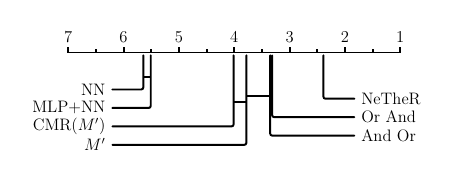
\begin{tikzpicture}[
  treatment line/.style={rounded corners=1.5pt, line cap=round, shorten >=1pt, line width=.5mm},
  treatment label/.style={font=\large},
  group line/.style={ultra thick},
  scale={0.5},
]

\begin{axis}[
  clip={false},
  axis x line={center},
  axis y line={none},
  axis line style={-},
  xmin={1},
  ymax={0},
  scale only axis={true},
  width={\axisdefaultwidth},
  ticklabel style={anchor=south, yshift=1.3*\pgfkeysvalueof{/pgfplots/major tick length}, font=\large},
  every tick/.style={draw=black, line width=.5mm},
  major tick style={yshift=.5*\pgfkeysvalueof{/pgfplots/major tick length}},
  minor tick style={yshift=.5*\pgfkeysvalueof{/pgfplots/minor tick length}},
  title style={yshift=\baselineskip},
  xmax={7},
  ymin={-4.5},
  height={5\baselineskip},
  xtick={1,2,3,4,5,6,7},
  minor x tick num={1},
  x dir={reverse},
]

\draw[treatment line] ([yshift=-2pt] axis cs:2.388888888888889, 0) |- (axis cs:1.8055555555555554, -2.5)
  node[treatment label, anchor=west] {NeTheR};
\draw[treatment line] ([yshift=-2pt] axis cs:3.3157894736842106, 0) |- (axis cs:1.8055555555555554, -3.5)
  node[treatment label, anchor=west] {Or And};
\draw[treatment line] ([yshift=-2pt] axis cs:3.3508771929824563, 0) |- (axis cs:1.8055555555555554, -4.5)
  node[treatment label, anchor=west] {And Or};
\draw[treatment line] ([yshift=-2pt] axis cs:3.780701754385965, 0) |- (axis cs:6.226608187134502, -5.0)
  node[treatment label, anchor=east] {$M'$};
\draw[treatment line] ([yshift=-2pt] axis cs:4.011695906432749, 0) |- (axis cs:6.226608187134502, -4.0)
  node[treatment label, anchor=east] {CMR($M'$)};
\draw[treatment line] ([yshift=-2pt] axis cs:5.508771929824562, 0) |- (axis cs:6.226608187134502, -3.0)
  node[treatment label, anchor=east] {MLP+NN};
\draw[treatment line] ([yshift=-2pt] axis cs:5.643274853801169, 0) |- (axis cs:6.226608187134502, -2.0)
  node[treatment label, anchor=east] {NN};
\draw[group line] (axis cs:3.780701754385965, -2.6666666666666665) -- (axis cs:4.011695906432749, -2.6666666666666665);
\draw[group line] (axis cs:5.508771929824562, -1.3333333333333333) -- (axis cs:5.643274853801169, -1.3333333333333333);
\draw[group line] (axis cs:3.3157894736842106, -2.3333333333333335) -- (axis cs:3.780701754385965, -2.3333333333333335);

\end{axis}
\end{tikzpicture}